
\chapter{Basic Graph Algorithm}

\section{Outline}
In this document, we will explore some fundamental algorithms and representations used in graph theory. We will cover the following topics:
\begin{itemize}
    \item How to represent graphs (Graph Representation)
    \item Breadth-First Search (BFS), a method for exploring graphs layer by layer
    \item Depth-First Search (DFS), which dives deeply into one branch before backtracking
    \item Directed Acyclic Graphs (DAGs), a special kind of directed graph with no cycles
\end{itemize}

\section{Graph Basics}
A graph is a structure that consists of two main components:
\begin{itemize}
    \item A set of vertices $V$ (also called nodes)
    \item A set of edges $E$, which connect pairs of vertices
\end{itemize}

Graphs can be used to model a wide range of real-world problems, from social networks to transportation systems. Let's break down some of the different types of graphs you might encounter.

\subsection{Types of Graphs}
Graphs can vary greatly in their structure and properties. Here are some important types:
\begin{itemize}
    \item \textbf{Undirected Graphs:} In an undirected graph, edges have no direction. This means if there is an edge between vertices $u$ and $v$, you can travel from $u$ to $v$ and vice versa. Formally, $(u, v) = (v, u)$. Self-loops (e.g. (v,v)) are not allowed.
    \item \textbf{Directed Graphs:} In directed graphs, edges have a specific direction. If there is an edge from $u$ to $v$, you cannot travel back from $v$ to $u$ unless a separate edge exists. This is written as $u \to v$. Self-loops are allowed.
    \item \textbf{Weighted Graphs:} In weighted graphs, each edge carries a value or cost, often representing distance or time. A weight function $w : E \to \mathbb{R}$ assigns a real number to each edge.
    \item \textbf{Dense and Sparse Graphs:} A graph is dense if it has a large number of edges, close to $|V|^2$. Conversely, a sparse graph has far fewer edges, often closer to $|V|$. $|E|$ = O($|V|^2$)
    \item \textbf{Connected Graphs:} A graph is \textbf{connected} if there is a path between every pair of vertices. In simpler terms, you can get from any vertex to any other vertex by following a series of edges. For a connected graph, the number of edges is at least $|V| - 1$. If the graph has exactly $|V| - 1$ edges and is connected, it forms a special structure called a tree.
\end{itemize}
When two vertices are connected by an edge, we say they are \textit{adjacent}. This relationship is symmetric in undirected graphs but not necessarily so in directed graphs.



\section{Graph Representation}
There are two main ways to represent graphs in computer programs: adjacency lists and adjacency matrices.

\begin{figure}[h]
    \centering
    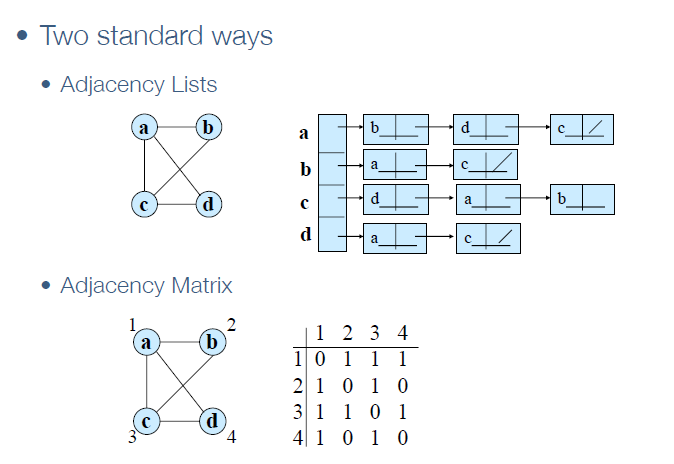
\includegraphics[width=0.75\linewidth]{graph representation.png}

\end{figure}

\subsection{Adjacency List Representation}
\begin{figure}[h!]
    \centering
    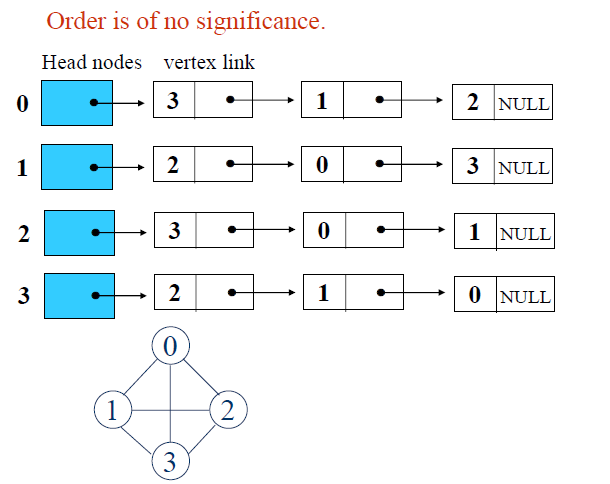
\includegraphics[width=0.75\linewidth]{adjacency list representation.png}

\end{figure}
Adjacency lists provide an efficient way to store graphs, especially when the graph is sparse. Here's how it works:
\begin{itemize}
    \item We maintain an array of lists, one for each vertex.
    \item Each list contains all the vertices adjacent to that vertex ( e.g. For u $\in V$, Adj[u] consists of all vertices adjacent to u).
    \item For directed graphs, the sum of the lengths of all adjacency lists equals the number of edges $|E|$. For undirected graphs, the sum is $2|E|$ because each edge appears in two lists.
    \item The storage requirement for adjacency lists is $\Theta(|V| + |E|)$.
\end{itemize}
This representation is space-efficient when the graph is sparse and has few edges relative to the number of vertices. \newline
The Cons of Adjacency Lists are:
\begin{itemize}
    \item Determining if an edge $(u,v) \in G$ is not efficient
    \item Have to search in u’s adjacency list. $\Theta(degree(u))$ time, $\Theta(V)$ in the worst case.
\end{itemize}

\subsection{Adjacency Matrix Representation}
An adjacency matrix is a more straightforward, but often less efficient, way to represent graphs:
\begin{itemize}
    \item We use a $|V| \times |V|$ matrix $A$.
        \[
        A[i, j] = 
        \begin{cases}
            1 & \text{if (i,j)$\in$ E} \\
            0 & \text{otherwise } 
        \end{cases}
        \]
    \item If there is an edge between vertices $i$ and $j$, then $A[i, j] = 1$. Otherwise, $A[i, j] = 0$.
    \item The matrix requires \textbf{ $\Theta(V^2)$ space}, which can be wasteful for large graphs with few edges.
    \item However, checking if an edge exists between two vertices takes constant time, $\Theta(1)$.
\end{itemize}
\begin{figure}[h!]
    \centering
    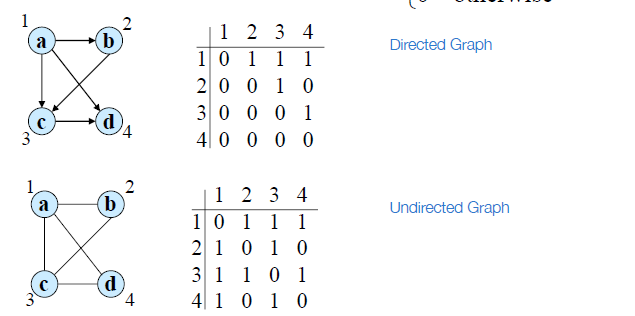
\includegraphics[width=0.75\linewidth]{Adjacency matrix.png}[h]

\end{figure}

\section{Graph Nomenclature}
Let's go over some basic terminology that will help when working with graphs:
\begin{itemize}
    \item A \textbf{path} of length $k$ from vertex $u$ to vertex $v$ in a graph=$G=(V,E)$ is a sequence of edges $p=<u,u1,u2, … , v> $ where $(u,u1)$, $(u1,u2)$ and
so on belongs to E; $|p|$ = k.
    \item Vertex $v$ is \textbf{reachable} from $u$ if there exists a path connecting them.
    \item A path is \textbf{simple} if no vertex is repeated.
    \item A graph is \textbf{strongly connected} if there is a path between every pair of vertices in both directions.
\end{itemize}
\section{Graph Search Algorithms}
\subsection{Breadth-First Search (BFS)}
Breadth-First Search (BFS) is one of the most fundamental graph traversal algorithms. It explores a graph layer by layer, starting from a specified source vertex $s\in V$.

\textbf{How BFS Works:}
\begin{itemize}
    \item We begin at vertex $s$ and mark it as discovered.
    \item All vertices directly connected to $s$ are discovered next.
    \item We continue exploring vertices one layer at a time until all reachable vertices are visited.
    \item BFS builds a tree rooted at $s$ that includes all reachable vertices.
\end{itemize}

\textbf{Key Outputs:}
\begin{itemize}
    \item $d[v]$: The shortest distance (in terms of the number of edges) from $s$ to $v$. If $v$ is not reachable from $s$, $d[v] = \infty$.
    \item $\pi[v]$: The predecessor of $v$ on the shortest path from $s$.
\end{itemize}

To keep track of progress during the search, vertices are colored:
\begin{itemize}
    \item White: Undiscovered
    \item Gray: Discovered but not finished
    \item Black: Finished
\end{itemize}
\begin{figure}[h]
    \centering
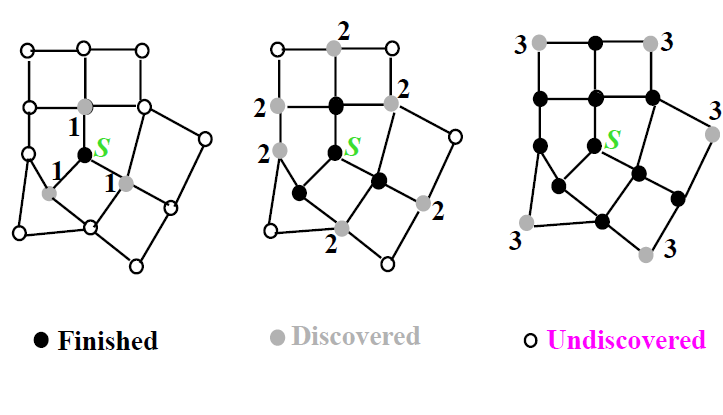
\includegraphics[width=0.75\linewidth]{Breadth-Firs-Search.png}

\end{figure}
BFS is useful for finding the shortest path in unweighted graphs and discovering the overall structure of a graph.

\newpage
\section{Breadth-First and Depth-First Search}

\textbf{Breadth-First Tree}
When performing a Breadth-First Search (BFS) on a graph $G = (V, E)$ starting from a source vertex $s$, we can construct a subgraph known as the \textbf{Breadth-First Tree}. This subgraph provides valuable insights into the shortest paths from $s$ to other vertices.

\subsection{Definition}
The predecessor subgraph $G_\pi$ of $G$ is defined as:
\begin{itemize}
    \item $V_\pi = \{v \in V : \pi[v] \neq \text{NIL}\} \cup \{s\}$
    \item $E_\pi = \{(\pi[v], v) \in E : v \in V_\pi - \{s\} \}$
\end{itemize}
In simpler terms:
\begin{itemize}
    \item $V_\pi$ contains all vertices reachable from $s$.
    \item $E_\pi$ contains edges that link each vertex to its predecessor.
\end{itemize}
The predecessor subgraph $G_\pi$ forms a Breadth-First Tree if:
\begin{itemize}
    \item $V_\pi$ consists of vertices reachable from $s$.
    \item For each $v \in V_\pi$, there exists a unique simple path from $s$ to $v$, which is also the shortest path in $G$.
\end{itemize}
The edges in $E_\pi$ are referred to as \textbf{tree edges}, and the tree will have $|E_\pi| = |V_\pi| - 1$ edges.

\section{BFS Algorithm and Analysis}
\subsection{BFS Pseudocode}
\textbf{BFS(G, s)}
\begin{figure}[h]
    \centering
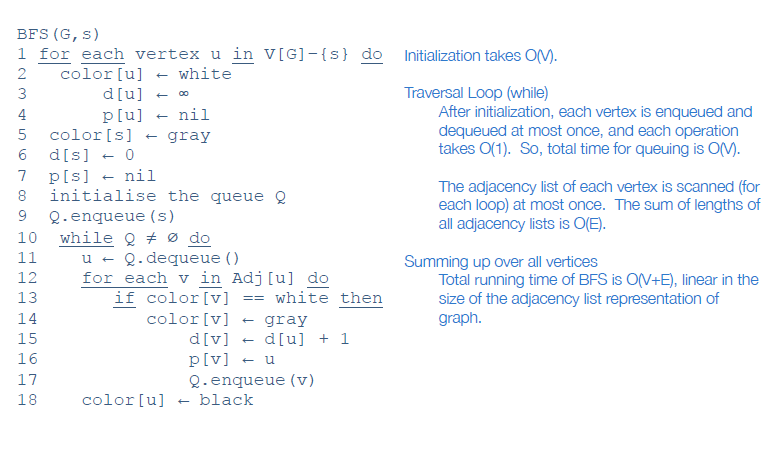
\includegraphics[width=1\linewidth]{BFS Pseudo code.png}

\end{figure}

\subsection{Analysis of BFS}
The BFS algorithm ensures that each vertex is enqueued and dequeued at most once. This results in a time complexity of $O(V)$ for queue operations. Additionally:
\begin{itemize}
    \item The adjacency list of each vertex is scanned at most once.
    \item Summing the lengths of all adjacency lists results in $O(E)$ operations.
    \item With the BFS method, we visit a number equal to the number of predecessors that discovered it, which corresponds to the in-degree.
\end{itemize}
Thus, the total running time of BFS is $O(V + E)$, which is linear with respect to the size of the graph.

\subsection{BFS:Example:}
\begin{figure}[h!]
    \centering
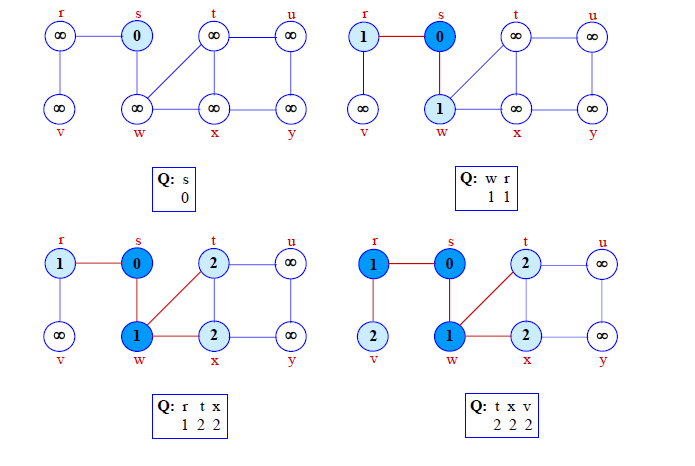
\includegraphics[width=0.75\linewidth]{BFS Ex. 1.png}
\end{figure}
\begin{figure} [h!]
    \centering
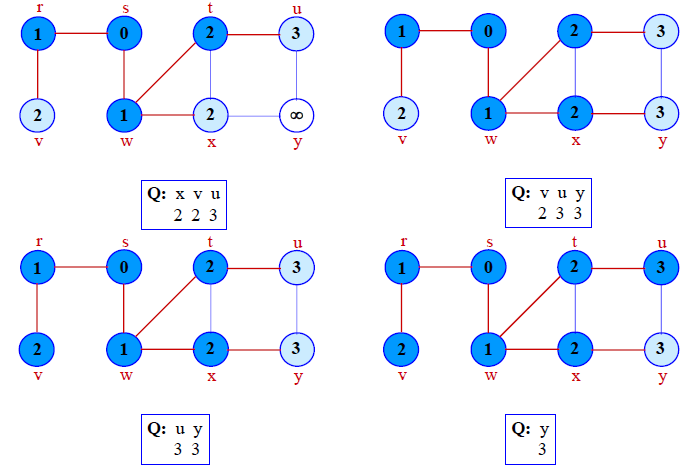
\includegraphics[width=0.75\linewidth]{BFS EX. 2.png}
\end{figure}
\newpage
\section{Depth-First Search (DFS)}

Depth-First Search (DFS) is a fundamental graph traversal algorithm used to explore all vertices and edges of a graph. The algorithm delves as deeply as possible along each branch before backtracking. It is particularly useful for tasks such as cycle detection, topological sorting, and connected component identification.

\subsection{Algorithm Overview}
The DFS algorithm explores edges out of the most recently discovered vertex \(v\). When all edges of \(v\) have been explored, it backtracks to the vertex from which \(v\) was discovered, continuing the process. This strategy embodies the principle: \emph{``Search as deep as possible first.''}

The process continues until all vertices reachable from the original source have been visited. If any undiscovered vertices remain, one of them is chosen as a new source, and the search is repeated.

\subsection{Input and Output}
\begin{itemize}
    \item \textbf{Input:} A graph \(G = (V, E)\), which can be directed or undirected. Unlike Breadth-First Search (BFS), no source vertex is specified initially.
    \item \textbf{Output:} 
    \begin{itemize}
        \item Two timestamps for each vertex:
        \begin{itemize}
            \item \(d[v]\): Discovery time, when \(v\) is first visited (color changes from white to gray).
            \item \(f[v]\): Finishing time, when the exploration of \(v\) is complete (color changes from gray to black).
        \end{itemize}
        \item \(\pi[v]\): Predecessor of vertex \(v\). For each vertex \(v\), \(\pi[v] = u\), where \(u\) is the vertex from which \(v\) was discovered.
    \end{itemize}
\end{itemize}

\subsection{Coloring Scheme}
DFS uses a coloring scheme to track the state of each vertex:
\begin{itemize}
    \item \textbf{White:} Vertex has not been discovered.
    \item \textbf{Gray:} Vertex has been discovered but is not yet fully explored.
    \item \textbf{Black:} Vertex and all its adjacent vertices have been fully explored.
\end{itemize}

\subsection{Key Steps of DFS}
\begin{enumerate}
    \item Initialize all vertices as white (unvisited), with \(\pi[v] = \text{NIL}\) and no timestamps.
    \item Start from an arbitrary vertex and mark it gray, recording its discovery time.
    \item Explore each unvisited adjacent vertex recursively.
    \item When all adjacent vertices of a vertex have been visited, mark it black and record its finishing time.
    \item Repeat the process for any remaining white vertices.
\end{enumerate}

\subsection{Applications of DFS}
DFS serves as the foundation for several advanced graph algorithms, including:
\begin{itemize}
    \item \textbf{Cycle detection:} Identifying cycles in directed or undirected graphs.
    \item \textbf{Topological sorting:} Ordering vertices in a Directed Acyclic Graph (DAG).
    \item \textbf{Connected components:} Finding connected subgraphs in an undirected graph.
    \item \textbf{Pathfinding:} Identifying paths between specific vertices.
\end{itemize}

\subsection{DFS Pseudocode}
The following pseudocode outlines the DFS algorithm:
\begin{verbatim}
DFS(G):
    for each vertex u in V[G]:
        color[u] ← white
        π[u] ← NIL
    time ← 0
    for each vertex u in V[G]:
        if color[u] == white:
            DFS-Visit(u)

DFS-Visit(u):
    color[u] ← gray
    time ← time + 1
    d[u] ← time
    for each v in Adj[u]:
        if color[v] == white:
            \pi[v] ← u
            DFS-Visit(v)
    color[u] ← black
    f[u] ← time
    time ← time + 1
\end{verbatim}

\subsection{Time Complexity}
The DFS algorithm operates in \(O(V + E)\) time for a graph \(G = (V, E)\) represented as an adjacency list. This efficiency arises because:
\begin{itemize}
    \item Each vertex is visited exactly once.
    \item Each edge is traversed at most twice (once for each vertex it connects).
\end{itemize}

\subsection{Classification of edges}
\begin{itemize}
    \item Tree edge: in the depth-first forest. Found by exploring (u, v). 
    \item Back edge: (u, v), where u is a descendant of v (in the depth-first tree). From v we can arrive to u. It is a back edge if the node is part of the tree and the edge leads to another node that is its ancestor.
    \item  Forward edge: (u, v), where v is a descendant of u, but not a tree edge. From v we can arrive in u but not in this case. It is a forward edge if the edge leads to a descendant that is not a tree edge.
    \item  Cross edge: any other edge. Can go between vertices in same depth-first tree or in different depth-first trees.
\end{itemize}

\subsection{DFS:EXAMPLE}
\begin{figure}[h]
    \centering
    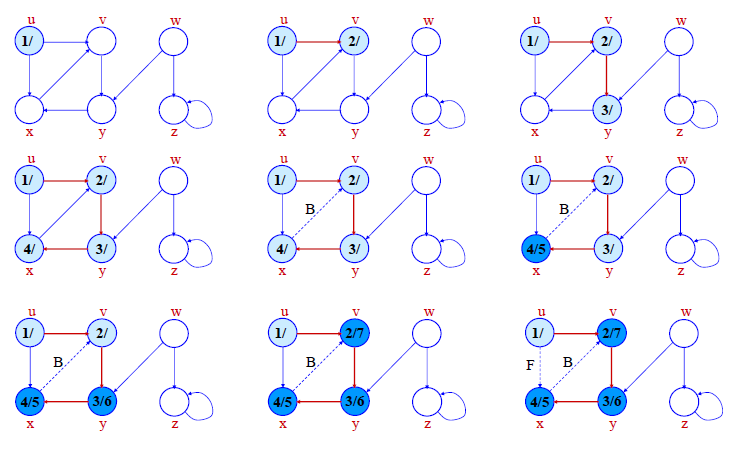
\includegraphics[width=0.75\linewidth]{DFS Example.png}
\end{figure}

\begin{figure}[h]
    \centering
    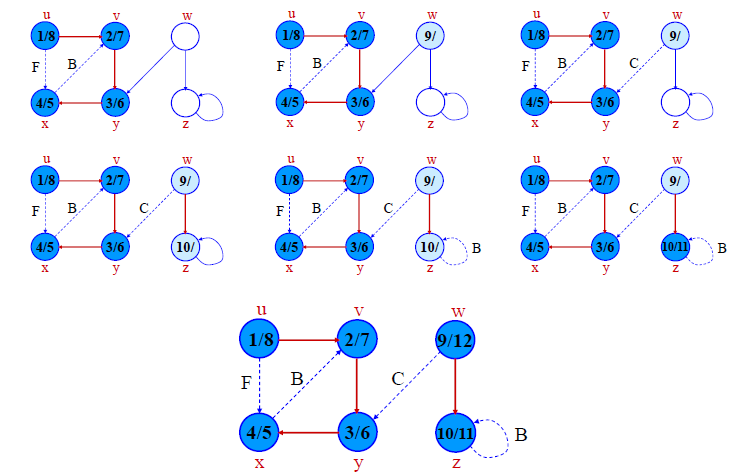
\includegraphics[width=0.75\linewidth]{DFS example 2.png}
\end{figure}
\newpage

\section{DFS Trees}
\begin{itemize}
    \item Predecessor subgraph defined slightly differently from that of BFS.
    \item The predecessor subgraph of DFS is \( G_{\pi} = (V_{\pi}, E_{\pi}) \) where
    \[
    E_{\pi} = \{ (\pi[v], v) : v \in V \text{ and } \pi[v] \neq \text{NIL} \}.
    \]
    \item The predecessor subgraph \( G_{\pi} \) forms a depth-first forest composed of several depth-first trees.
    \item The edges in \( E_{\pi} \) are called tree edges.
\end{itemize}

\section{Graph Algorithms:Single Source Shortest Path}
The Shortest Path algorithm calculates the shortest (weighted) path between a pair of nodes. It’s useful for user interactions and dynamic workflows because it works in real time. $\\$
Use Shortest Path to find optimal routes between a pair of nodes, based on either the number of hops or any weighted relationship value.
It can provide real-time answers about degrees of separation, the shortest distance between points, or the least expensive route.$\\$
Let \( G = (V, E) \) be a weighted graph such that there exists a weight function \( w : E \to \mathbb{R} \).  
We define a direct path from \( v_1 \) to \( v_k \), denoted \( v_1 \rightsquigarrow v_k \), as  
\[ p = v_1 \to v_2 \to \dots \to v_{k-1} \to v_k. \]  
The weight of \( p \) is given by  
\[ w(p) = \sum_{i=1}^{k-1} w(v_i, v_{i+1}). \]  
The weights can be negative, positive, or zero.  

The shortest path from \( u \) to \( v \) is the path \( p_{u,v} \) with minimum weight. A simplification of this problem is to calculate the weight of the shortest path rather than the path itself. We denote the shortest path weight as  
\[ \delta(u, v) = \min \{ w(p) : p \text{ is a path from } u \text{ to } v \}. \]

\subsection{Dijkstra Algorithm (GREEDY)}
Dijkstra’s Shortest Path algorithm operates by first finding the lowest-weight relationship from the start node to directly connected nodes. It keeps track of those weights and moves to the “closest” node.  It then performs the same calculation, but now as a cumulative total from the start node. The algorithm continues to do this, evaluating a “wave” of cumulative weights and always choosing the lowest weighted cumulative path to advance along, until it reaches the destination node.
\newline
The complexity is $O(n^2)$ if we start from an array.

\begin{figure}[H]
    \centering
    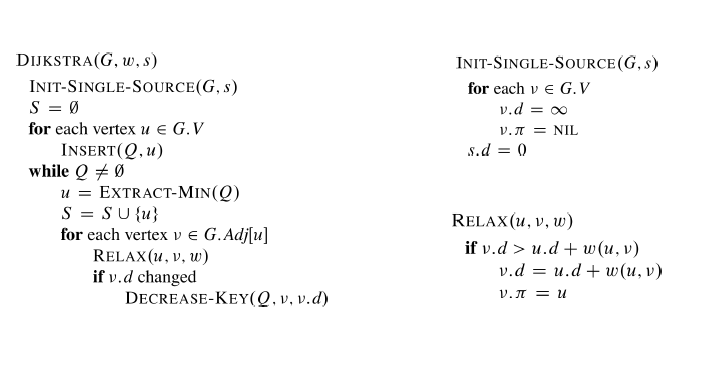
\includegraphics[width=0.75\linewidth]{dijkstra algorithm .png}
\end{figure}
\subsection{Dijkstra exercise}
\paragraph{How does it work?} I start with a set $Q$, a list of my nodes along with their initialization. I begin with the smallest node and extract it from the list; this node can no longer be directly considered for modifying its adjacent nodes. Taking a node $x$, I update its neighbors $y$. If $x.\text{value} + w(x, y)$ (the weight between $x$ and $y$) is smaller than $y.\text{value}$, then $y.\text{value} = x.\text{value} + w(x, y)$. I then move to the node with the smallest value and repeat the process. When $Q$ is empty, I stop. It is important to note that even though I follow the smallest path, I update all nodes that can be updated.
\newpage
\begin{figure}[H]
    \centering
    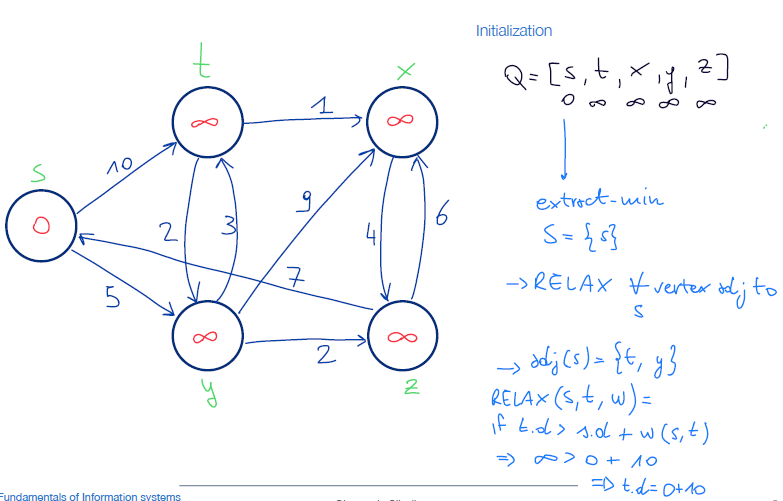
\includegraphics[width=0.75\linewidth]{dij ex 1.png}

\end{figure}

\begin{figure}[H]
    \centering
    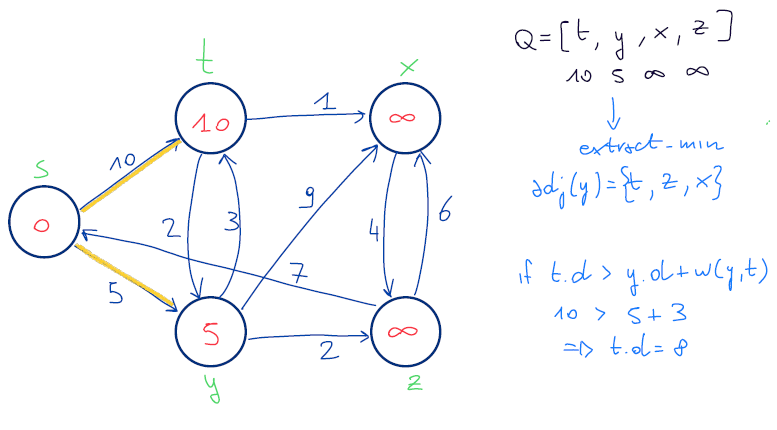
\includegraphics[width=0.75\linewidth]{dij ex 2.png}

\end{figure}

\begin{figure}[H]
    \centering
    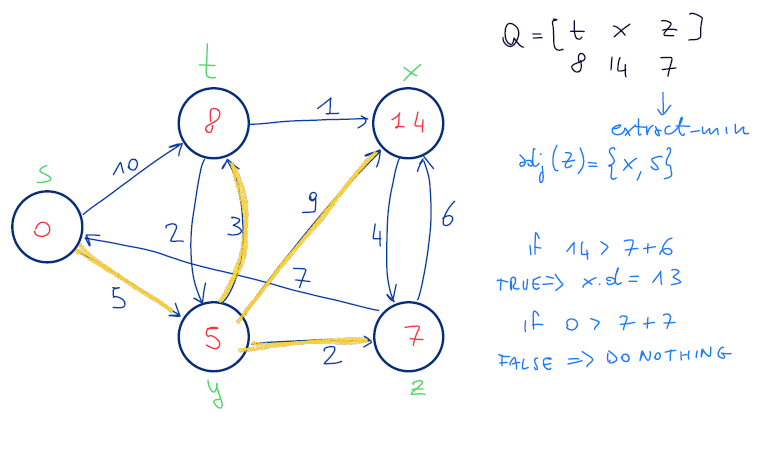
\includegraphics[width=0.75\linewidth]{dij ex 3.png}

\end{figure}

\begin{figure}[H]
    \centering
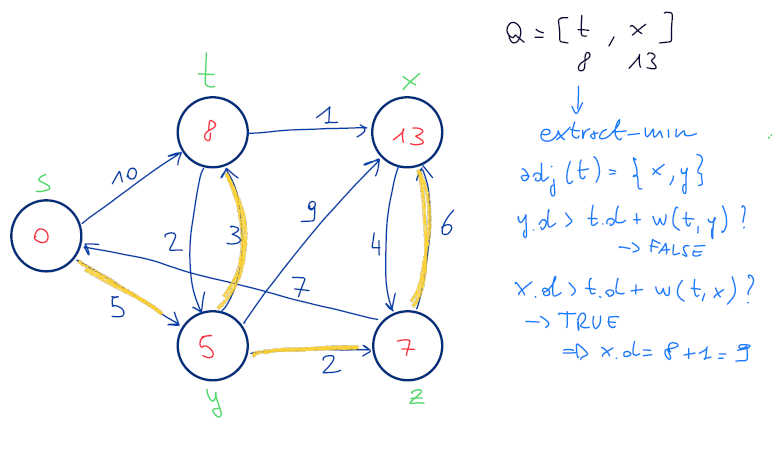
\includegraphics[width=0.75\linewidth]{dij ex 4.png}

\end{figure}
\begin{figure}[H]
    \centering
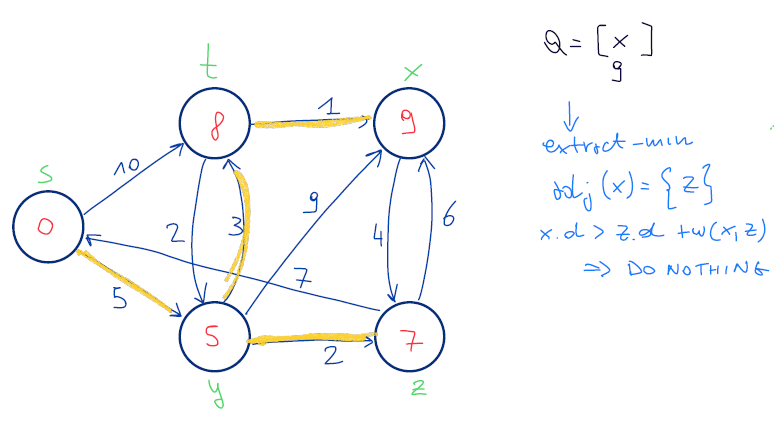
\includegraphics[width=0.75\linewidth]{dij ex 5.png}

\end{figure}
\begin{figure}[H]
    \centering
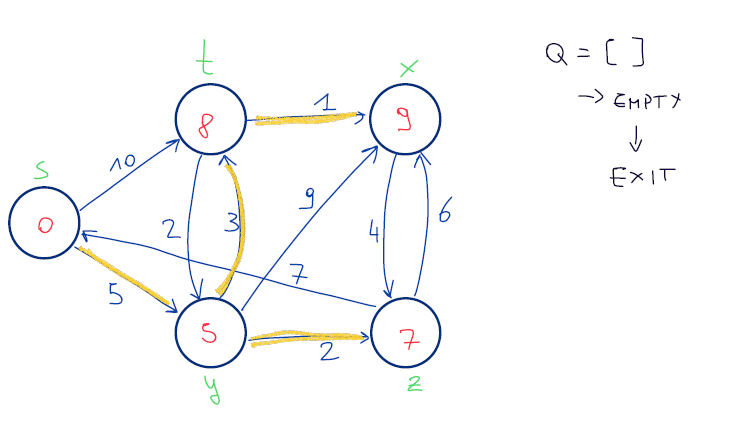
\includegraphics[width=0.75\linewidth]{dij ex 6.png}

\end{figure}



\section{Graph Algorithms: Properties and Concepts}

The Single Source Shortest Path (SSSP) problem is fundamental in graph theory and provides insights into various properties that help solve it efficiently:

\begin{itemize}
    \item \textbf{Triangle Inequality:} For any edge $(u,v) \in E$, the inequality \( \delta(s,v) \leq \delta(s,u) + w(u,v) \) holds, where \( \delta(s,v) \) represents the shortest path distance from source \( s \) to \( v \).
    
    \item \textbf{Upper-Bound Property:} For all vertices \( v \in V \), we always have \( v.d \geq \delta(s,v) \). Once \( v.d \) reaches the value \( \delta(s,v) \), it does not change.

    \item \textbf{No-Path Property:} If there is no path between the source \( s \) and a vertex \( v \), then \( v.d = \delta(s,v) = \infty \).

    \item \textbf{Convergence Property:} If a shortest path \( s \to u \to v \) exists in \( G \) for vertices \( u \) and \( v \), and \( u.d = \delta(s,u) \) before relaxing edge \( (u,v) \), then \( v.d = \delta(s,v) \) after the relaxation.
\end{itemize}

\section{Minimum Spanning Tree (MST)}

Given a weighted graph \( G(V, E) \) with edge weights \( w: E \to \mathbb{R} \), a Minimum Spanning Tree is a subgraph that:
\begin{itemize}
    \item Connects all vertices in \( G \).
    \item Minimizes the total weight of the edges.
\end{itemize}

The first known algorithm for MST was developed by Otakar Bor\u{u}vka in 1926, followed by Prim's algorithm in 1957, which is widely used and resembles Dijkstra's algorithm but focuses on minimizing individual edge weights.

\subsection{Prim's Algorithm (GREEDY)}
Prim's algorithm starts from an arbitrary node and grows the MST iteratively:
\begin{enumerate}
    \item Begin with a tree containing one node.
    \item Add the edge with the smallest weight that connects a new node to the tree.
    \item Repeat until all nodes are included.
\end{enumerate}
\begin{figure}[H]
    \centering
    \includegraphics[width=0.75\linewidth]{Prim's MSt: main Steps.png}

\end{figure}

\subsection{Prim's Algorithm: Pseudo-Code}
 \begin{figure}[H]
     \centering
     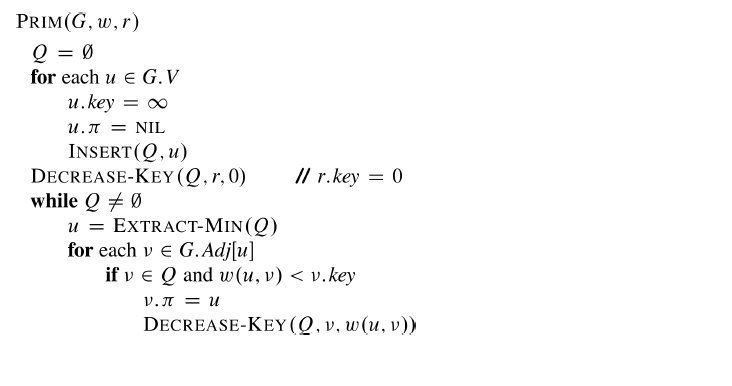
\includegraphics[width=0.75\linewidth]{Prim's MSt pseudo.png}

 \end{figure}


\subsection{Applications of MST}
\begin{itemize}
    \item Optimal routing in scenarios where all nodes must be visited, such as network design.
    \item Approximation for problems like the Traveling Salesman Problem (TSP).
\end{itemize}

\section{Centrality Algorithms}

Centrality algorithms measure the importance of nodes within a graph. They provide insights into network dynamics such as influence, accessibility, and information flow.

\subsection{Types of Centrality Measures}
\begin{itemize}
    \item \textbf{Degree Centrality:} Counts the number of edges connected to a node. High degree centrality indicates popularity or influence.
    \item \textbf{Closeness Centrality:} Measures the average shortest path from a node to all others. Nodes with high closeness centrality are efficient at spreading information.
    \item \textbf{Betweenness Centrality:} Counts the number of shortest paths passing through a node, identifying nodes critical for information flow.
    \item \textbf{PageRank:} Evaluates a node's importance based on its neighbors and their connections.
\end{itemize}

\begin{figure}[H]
    \centering
    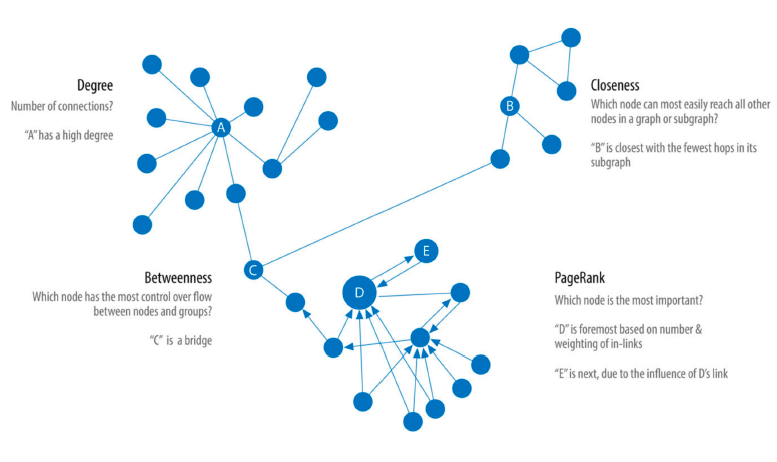
\includegraphics[width=0.75\linewidth]{centrality algorithms.png}

\end{figure}

\subsection{Formulas for Centrality Measures}
\begin{itemize}
    \item \textbf{Normalized Closeness Centrality:}
    \[
    C_{\text{norm}}(u) = \frac{n-1}{\sum_{v=1}^{n-1} \delta(u,v)}
    \]
    where \( \delta(u,v) \) is the shortest path between \( u \) and \( v \).
    \begin{figure}[H]
        \centering
        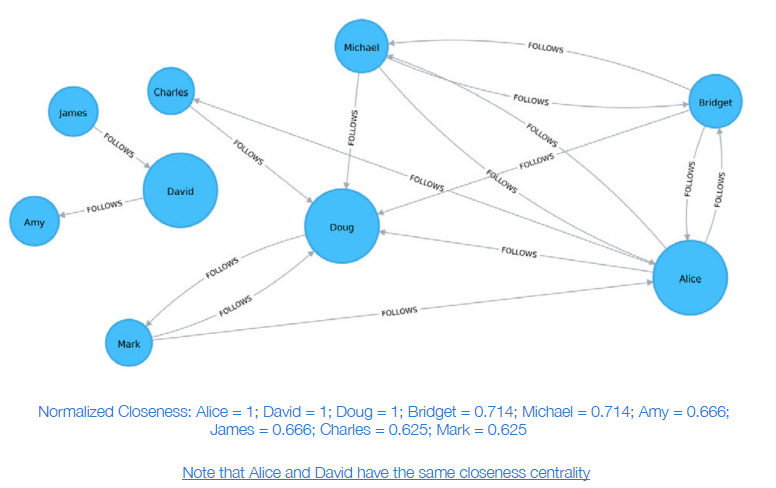
\includegraphics[width=0.75\linewidth]{image.png}
    
    \end{figure}
    
    \item \textbf{Wasserman-Faust Closeness Centrality:}
    \[
    C_{\text{WF}}(u) = \left(\frac{n-1}{N-1}\right) \cdot \left(\frac{n-1}{\sum_{v=1}^{n-1} \delta(u,v)}\right)
    \]
\begin{figure}[H]
    \centering
    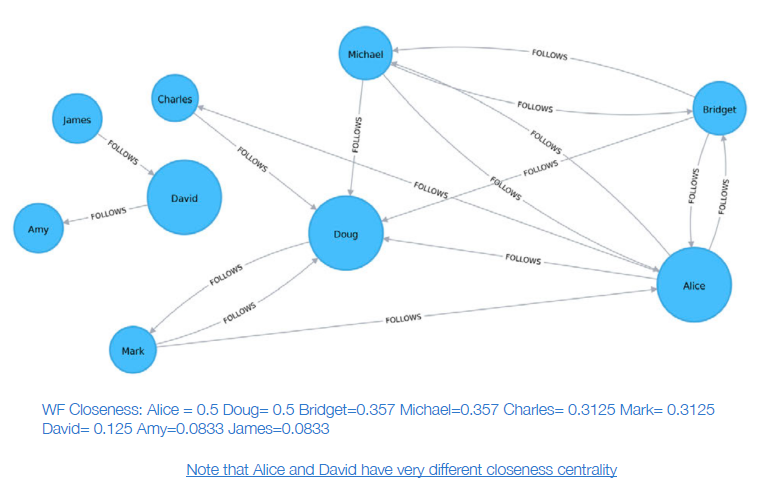
\includegraphics[width=0.75\linewidth]{wes and f closs cent.png}

\end{figure}

    \item \textbf{Harmonic Centrality:}
    \[
    H(u) = \frac{\sum_{v=1}^{n-1} \frac{1}{\delta(u,v)}}{N-1}
    \]
\end{itemize}
\begin{figure}[H]
    \centering
    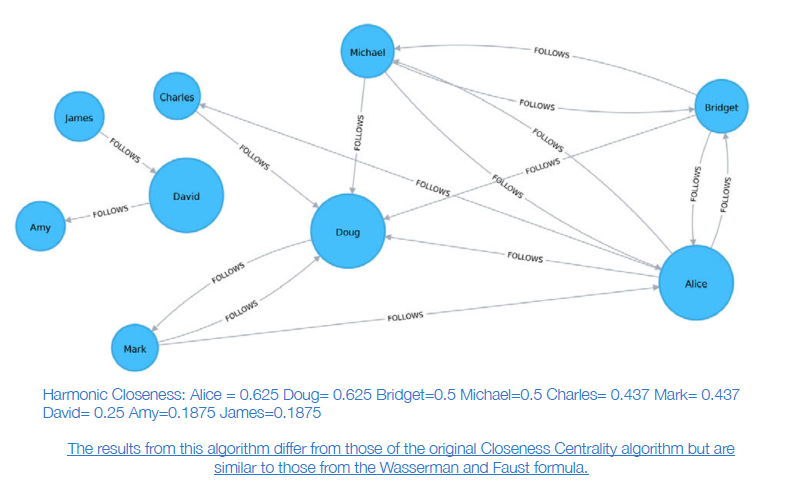
\includegraphics[width=0.75\linewidth]{Harmonic cent.png}

\end{figure}


\section{Conclusion}

Understanding graph algorithms and their properties is essential for solving problems related to network optimization, data flow, and centrality in complex systems. By applying these algorithms effectively, one can extract valuable insights and design efficient solutions in various domains.

\section{Betweenness Centrality}
\begin{figure}[h!]
    \centering
    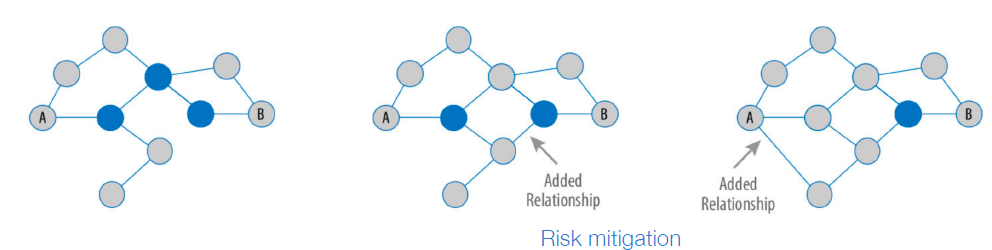
\includegraphics[width=0.75\linewidth]{immagini/betcentr.png}
\end{figure}
Betweenness Centrality is a measure used to determine the influence a node exerts over the flow of information or resources within a graph. It helps identify nodes that serve as bridges, connecting different parts of the graph. This property is essential in understanding network dynamics and potential vulnerabilities.

The \textbf{Betweenness Centrality } algorithm works by calculating the shortest paths between all pairs of nodes in a connected graph. Each node receives a score based on the number of these shortest paths that pass through it. Nodes lying on a significant number of shortest paths are assigned higher scores.

A node is pivotal for two other nodes if it lies on every shortest path between them. Removing a pivotal node increases the cost or length of the shortest paths, highlighting its critical role in maintaining connectivity. Bridges in a graph, whether nodes or relationships, are crucial to network integrity. For example, removing a bridge might disconnect parts of the graph.

The formal definition of Betweenness Centrality for a node \( u \) in a graph \( G(V,E) \), where \( |V| = N \), is:
\[B(u) = \sum_{s \neq u \neq t} \frac{p(u)}{p},\]
where \( p(u) \) is the number of shortest paths between nodes \( s \) and \( t \) that pass through \( u \), and \( p \) is the total number of shortest paths between \( s \) and \( t \).

To compute Betweenness Centrality:
\begin{enumerate}
    \item Identify all shortest paths in the graph.
    \item Count the fraction of these paths that pass through each node.
    \item Sum these fractions to determine the node's Betweenness Centrality score.
\end{enumerate}

\textbf{Applications:}
\begin{itemize}
    \item Identifying key influencers in organizations, especially those in brokerage positions.
    \item Locating critical transfer points in networks like electrical grids.
    \item Designing strategies for spreading influence effectively on social platforms.
\end{itemize}

\section{PageRank}
PageRank is a widely recognized centrality algorithm that measures the transitive influence of nodes in a network. Unlike other algorithms that focus on direct influence, PageRank evaluates the influence of a node’s neighbors and their neighbors.

The algorithm was developed by Larry Page and is the foundation of Google’s search ranking system. Its core assumption is that a node with more incoming relationships, particularly from influential neighbors, is more credible.

The PageRank of a node \( u \) is defined recursively:
\[
PR(u) = (1 - d) + d \left[ \frac{PR(T_1)}{C(T_1)} + \cdots + \frac{PR(T_n)}{C(T_n)} \right],
\]
where:
\begin{itemize}
    \item \( d \) is the damping factor, typically set to 0.85, representing the probability that a user follows a link rather than navigating randomly.
    \item \( 1 - d \) represents the probability of landing directly on a page.
    \item \( C(T_n) \) is the out-degree of node \( T_n \), the number of links it provides.
\end{itemize}

PageRank iteratively updates the rank of each node until the values converge or a predefined number of iterations is reached. Conceptually, it assumes a web surfer navigating links or visiting random URLs. The damping factor mitigates issues like rank sinks (nodes without outgoing links) by introducing teleportation to random nodes.

\textbf{Challenges and Strategies:}
\begin{itemize}
    \item \textit{Rank sinks:} Nodes or subsets without outgoing links monopolize PageRank scores. To address this, outgoing relationships to all nodes are assumed, allowing teleportation.
    \item \textit{Circular references:} Nodes pointing exclusively to each other inflate their ranks. The damping factor mitigates this by introducing a probability for random visitation.
\end{itemize}

\textbf{Applications:}
\begin{itemize}
    \item Ranking web pages by relevance in search engines.
    \item Identifying influential nodes in social and communication networks.
    \item Prioritizing features in machine learning models.
\end{itemize}

\subsection{exercise}
\begin{figure}[h!]
    \centering
    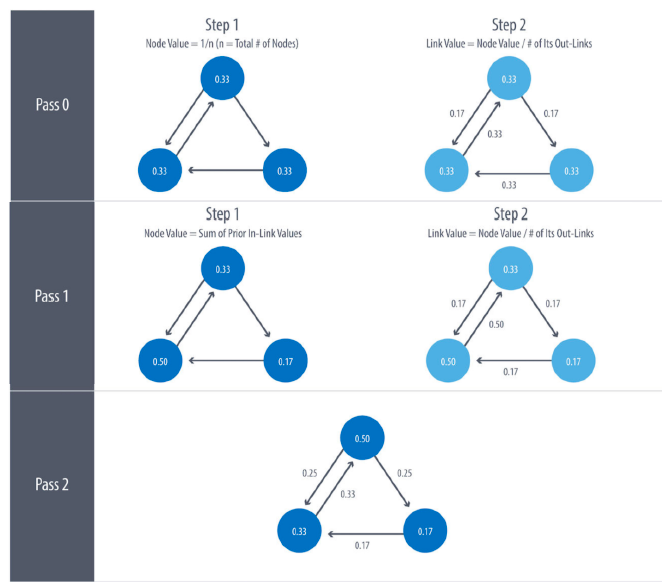
\includegraphics[width=0.75\linewidth]{immagini/pagerank.png}
\end{figure}

\newpage

%%% questo è quello che abbiamo fatto l'ultima lezione fa sempre parte dei graphs, lo metto qui in fondo

